\section{Условие задания}

\begin{figure}[H]
    \begin{center}
        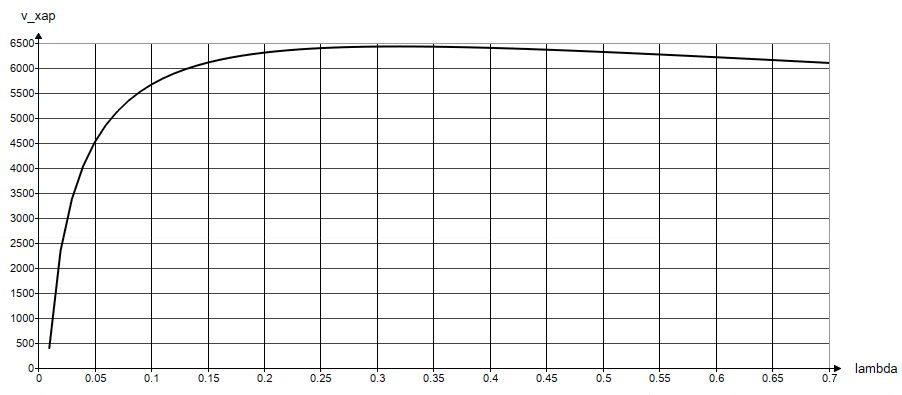
\includegraphics[width = 0.5\linewidth]{pic1.PNG}
        \caption{Условие задания}
        \label{pic1}
    \end{center}
\end{figure}

В данном задании необходимо определить перемещения в кольце $v$ и $w$.

\section{Решение}

Из предыдущего домашнего задания имеем следующие выражения:
\begin{itemize}
    \item Уравновешивающая нагрузка:
    \begin{equation}
        \label{eq0}
        t = \frac{4q_0}{\pi} \sin \phi
    \end{equation}
    \item Момент на кольце:
    \begin{equation}
        \label{eq0.1}
        \begin{cases}
            \displaystyle M_1 = q_0R^2 \left( 1 - \frac{3}{\pi} \cos \phi - \frac{2}{\pi} \phi \sin \phi \right)
            \\[10pt]
            \displaystyle M_2 = q_0R^2 \left( 2 \sin \phi - \frac{3}{\pi} \cos \phi - \frac{2}{\pi} \phi \sin \phi - 1 \right)
        \end{cases}
    \end{equation}
\end{itemize}

Запишем разрешающее уравнение кольца:
\begin{equation}
    \label{eq1}
    \frac{d^6 v}{d \phi^6} + 2\frac{d^4 v}{d \phi^4} + \frac{d^2 v}{d \phi^2} = - \frac{R^3}{EJ} \left[ R \left( t + \frac{dQ}{d \phi} \right) + \left( \frac{d^2 m}{d \phi^2} + m \right) \right]
\end{equation}

Решение этого уравнения имеет вид:
\begin{equation}
    \label{eq2}
    v = A_0 + \sum_{n = 1}^{\infty} \left( A_n \cos n \phi + B_n \sin n \phi \right)
\end{equation}

Коэффициенты можно найти по формулам:
\begin{equation}
    \label{eq3}
    \begin{cases}
        \displaystyle A_n = \frac{R^4}{EJn^2(n^2-1)^2} \left[ a_n'' + nb_n' - \frac{1}{R}(n^2 - 1)a_n''' \right]
        \\[10pt]
        \displaystyle B_n = \frac{R^4}{EJn^2(n^2 - 1)^2} \left[ b_n'' - na_n' - \frac{1}{R}(n^2 - 1)b_n''' \right]
    \end{cases}
\end{equation}

Коэффициент $A_0$ задает перемещение всего кольца как одно целое, поэтому задаем его равным $A_0 = 0$.

Коэффициенты в формуле (\ref{eq3}) можно найти по формулам:
\begin{equation}
    \label{eq4}
    \left\{
        \begin{array}{lr}
            a_n'
            \\
            a_n''
            \\
            a_n'''
        \end{array}
    \right\}
    = \frac{1}{\pi} \int_{0}^{2\pi}
    \left\{ 
        \begin{array}{lr}
            q_n
            \\
            q_t
            \\
            m
        \end{array}
    \right\}
    \cos n \phi d \phi
\end{equation}

\begin{equation}
    \label{eq5}
    \left\{
        \begin{array}{lr}
            b_n'
            \\
            b_n''
            \\
            b_n'''
        \end{array}
    \right\}
    = \frac{1}{\pi} \int_{0}^{2\pi}
    \left\{ 
        \begin{array}{lr}
            q_n
            \\
            q_t
            \\
            m
        \end{array}
    \right\}
    \sin n \phi d \phi
\end{equation}

В нашем случае распределенная нагрузка равна:
\begin{equation}
    \label{eq6}
    q_{n} = q_0, \;\; \phi < \frac{\pi}{2}, \; \phi > \frac{3\pi}{2}
\end{equation}
\begin{equation}
    \label{eq7}
    q_t = t + q_{t1} + q_{t2}
\end{equation}
\begin{equation}
    \label{eq8}
    m = 0
\end{equation}

Распределим сосредоточенную нагрузку $q_0R$:
\begin{equation}
    \label{eq9}
    q_{ti} = \frac{q_0R}{\pi R} \left[ \frac{1}{2} + \sum_{n = 1}^{\infty} \left( \cos n (\phi - \phi_0) \right) \right]
\end{equation}
\begin{equation}
    \label{eq10}
    q_{t1} = -\frac{q_0}{\pi} \left[ \frac{1}{2} + \sum_{n = 1}^{\infty} \left( \cos n (\phi - \frac{\pi}{2}) \right) \right]
\end{equation}
\begin{equation}
    \label{eq11}
    q_{t2} = \frac{q_0}{\pi} \left[ \frac{1}{2} + \sum_{n = 1}^{\infty} \left( \cos n (\phi + \frac{\pi}{2}) \right) \right]
\end{equation}

Получим:
\begin{equation}
    \label{eq12}
    \begin{split}
        q_t & = \frac{4q_0}{\pi} \sin \phi - \frac{q_0}{\pi} \left[ \frac{1}{2} + \sum_{n = 1}^{\infty} \left( \cos n (\phi - \frac{\pi}{2}) \right) \right] + \frac{q_0}{\pi} \left[ \frac{1}{2} + \sum_{n = 1}^{\infty} \left( \cos n (\phi + \frac{\pi}{2}) \right) \right] =
        \\
        & = \frac{q_0}{\pi} \left( 4 \sin \phi + \sum_{n = 1}^{\infty} \left( -\cos n \frac{\pi}{2} \cos n \phi - \sin n \frac{\pi}{2} \sin n \phi + \cos n \frac{\pi}{2} \cos n \phi - \sin n \frac{\pi}{2} \sin n \phi \right) \right) =
        \\
        & = \frac{q_0}{\pi} \left( 4 \sin \phi - 2\sum_{n = 1}^{\infty} \sin\frac{\pi n}{2} \sin n \phi \right)
    \end{split}
\end{equation}

Получим следующие выражения для коэффициентов (\ref{eq4}) и (\ref{eq5}):
\begin{equation}
    \label{eq12.1}
    \begin{split}
        a_n' & = \frac{1}{\pi} \left( \int_{0}^{\frac{\pi}{2}} q_0 \cos n\phi d\phi + \int_{\frac{3\pi}{2}}^{2\pi} q_0\cos n\phi d\phi \right) = \frac{q_0}{\pi n} \left( \sin n \phi \big|_{0}^{\frac{\pi}{2}} + \sin n \phi \big|_{\frac{3\pi}{2}}^{2\pi} \right) = 
        \\
        & = \frac{q_0}{\pi n} \left( \sin \frac{\pi n}{2} - \sin \frac{3\pi n}{2} \right) = \frac{2q_0}{\pi n} \sin \frac{\pi n}{2}
    \end{split}
\end{equation}
\begin{equation}
    \label{eq12.2}
    \begin{split}
        b_n' & = \frac{1}{\pi} \left( \int_{0}^{\frac{\pi}{2}} q_0 \sin n\phi d\phi + \int_{\frac{3\pi}{2}}^{2\pi} q_0 \sin n\phi d\phi \right) = -\frac{q_0}{\pi n} \left( \cos n\phi \big|_{0}^{\frac{\pi}{2}} + \cos n\phi \big|_{\frac{3\pi}{2}}^{2\pi} \right) =
        \\
        & = -\frac{q_0}{\pi n} \left( \cos \frac{\pi n}{2} - 1 + 1 - \cos \frac{3\pi n}{2} \right) = -\frac{q_0}{\pi n} \left( \cos \frac{\pi n}{2} - \cos \frac{\pi n}{2} \right) = 0
    \end{split}
\end{equation}
\begin{equation}
    \label{eq12.3}
    \begin{split}
        a_n'' & = \frac{1}{\pi} \int_{0}^{2\pi} \frac{q_0}{\pi} \left( 4\sin \phi - 2 \sum_{k=1}^{\infty} \sin \frac{\pi k}{2} \sin k\phi \right) \cos n\phi d\phi =
        \\
        & = \frac{q_0}{\pi^2} \left( 4\int_{0}^{2\pi} \sin\phi \cos n\phi d\phi - 2\sum_{k=1}^{\infty} \sin \frac{\pi k}{2} \int_{0}^{2\pi} \sin k\phi \cos n\phi d\phi \right) = 0
    \end{split}
\end{equation}
\begin{equation}
    \label{eq12.4}
    \begin{split}
        b_n'' & = \frac{1}{\pi} \int_{0}^{2\pi} \frac{q_0}{\pi} \left( 4\sin \phi - 2 \sum_{k=1}^{\infty} \sin \frac{\pi k}{2} \sin k\phi \right) \sin n\phi d\phi =
        \\
        & = \frac{q_0}{\pi^2} \left( 4\int_{0}^{2\pi} \sin\phi \sin n\phi d\phi - 2\sum_{k=1}^{\infty} \sin \frac{\pi k}{2} \int_{0}^{2\pi} \sin k\phi \sin n\phi d\phi \right) = 
        \\
        & = \frac{q_0}{\pi^2} \left( 4\int_{0}^{2\pi} \sin \phi \sin n\phi d\phi - 2\sin \frac{\pi n}{2} \int_{0}^{2\pi} \sin^2 n\phi d\phi \right)
        \\
        & = 
        \begin{cases}
            \displaystyle \frac{q_0}{\pi^2} \left( 4\pi - 2\pi \sin \frac{\pi}{2} \right) = \frac{2q_0}{\pi}, \; n = 1
            \\[10pt]
            \displaystyle -\frac{2q_0}{\pi} \sin \frac{\pi n}{2}, \; n \neq 1
        \end{cases}
    \end{split}
\end{equation}
\begin{equation}
    \label{eq12.5}
    \begin{cases}
        a_n''' = 0
        \\
        b_n''' = 0
    \end{cases}
\end{equation}

Проверим полученные коэффициенты с помощью выражений:
\begin{equation}
    \label{eq12.5.1}
    \begin{cases}
        B - a_1'' + b_1' = 0
        \\
        C - b_1'' - a_1' = 0
    \end{cases}
\end{equation}
\begin{equation}
    \label{eq12.5.2}
    0 - 0 + 0 = 0
    \\
    \frac{4q_0}{\pi} - \frac{2q_0}{\pi} - \frac{2q_0}{\pi} = 0
\end{equation}
Условия (\ref{eq12.5.1}) выполняются, значит коэффициенты найдены правильно.

Получим коэффициенты разложения (\ref{eq3}):
\begin{equation}
    \label{eq12.6}
    A_n = 0
\end{equation}
\begin{equation}
    \label{eq12.7}
    B_n = \frac{R^4}{EJn^2(n^2 - 1)^2} \left[ -\frac{2q_0}{\pi} \sin \frac{\pi n}{2} -n \frac{2q_0}{\pi n} \sin \frac{\pi n}{2} \right] = -\frac{4q_0R^4}{\pi EJn^2(n^2 - 1)^2} \sin \frac{\pi n}{2}
\end{equation}

Получим следующее разложение функции касательных перемещений:
\begin{equation}
    \label{eq12.8}
    v = -\frac{4q_0R^4}{\pi EJ} \sum_{n=2}^{\infty} \frac{1}{n^2(n^2 - 1)^2} \sin \frac{\pi n}{2} \sin n\phi
\end{equation}

Примем количество членов ряда (\ref{eq2}) равным $N = 50$. Построим эпюры перемещений и изгибающего момента:
\begin{figure}[H]
    \begin{center}
        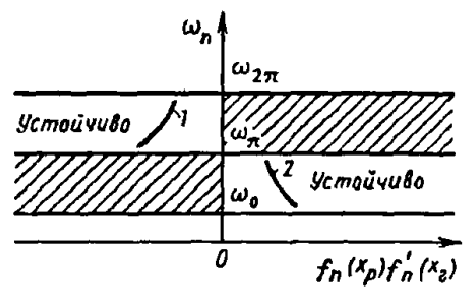
\includegraphics[width = 0.8\linewidth]{pic2.PNG}
        \caption{Эпюра касательных перемещений}
        \label{pic2}
    \end{center}
\end{figure}

Найдем нормальные перемещения:
\begin{equation}
    \label{eq13}
    w = - \frac{dv}{d\phi} = \frac{4q_0R^4}{\pi EJ} \sum_{n=2}^{\infty} \frac{1}{n(n - 1)^2(n + 1)^2} \sin \frac{\pi n}{2} \cos(n \phi)
\end{equation}

\begin{figure}[H]
    \begin{center}
        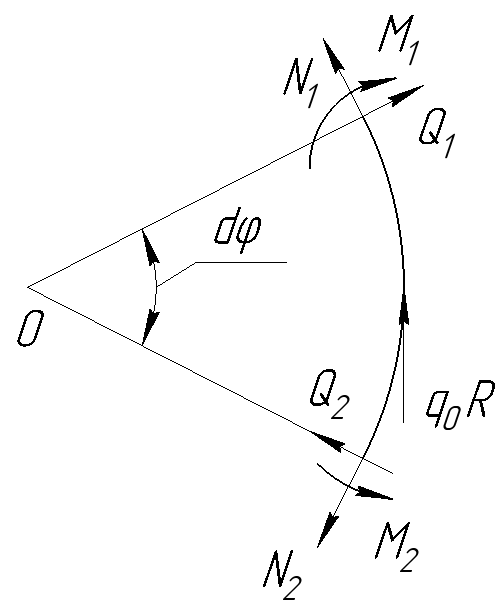
\includegraphics[width = 0.8\linewidth]{pic3.PNG}
        \caption{Эпюра нормальных перемещений}
        \label{pic3}
    \end{center}    
\end{figure}

Найдем изгибающий момент:
\begin{equation}
    \label{eq14}
    M = \frac{EJ}{R^2} \left(\frac{d^2 w}{d \phi^2} + w \right) = -\frac{4q_0R^2}{\pi} \sum_{n=2}^{\infty} \frac{1}{n(n^2 - 1)} \sin \frac{\pi n}{2} \cos n\phi
\end{equation}

\begin{figure}[H]
    \begin{center}
        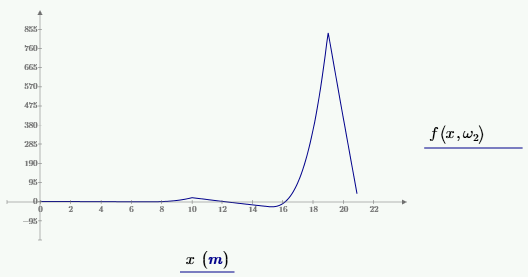
\includegraphics[width = 0.8\linewidth]{pic4.PNG}
        \caption{Эпюра изгибающего момента}
        \label{pic4}
    \end{center}
\end{figure}

Сплошной линией обозначено текущее решение $M_2(\phi)$, а прерывистой --- аналитическое решение из прошлого задания $M_1(\phi)$. Для сравнения возьмем значения моментов в нескольких точках:
\begin{itemize}
    \item $\phi = 0: \; M_1(0) = 0.0451; \; M_2(0) = 0.0451$
    \item $\displaystyle \phi = \frac{\pi}{4}: \; M_1(\frac{\pi}{4}) = -0.02879; \; M_2(\frac{\pi}{4}) = -0.02891$
    \item $\displaystyle \phi = \frac{\pi}{2}: \; M_1(\frac{\pi}{2}) = 0; \; M_2(\frac{\pi}{2}) = 0.00003$
    \item $\displaystyle \phi = \frac{3\pi}{4}: \; M_1(\frac{3\pi}{4}) = 0.02879; \; M_2(\frac{3\pi}{4}) = 0.02889$
    \item $\displaystyle \phi = \pi: \; M_1(\pi) = -0.04507; \; M_2(\pi) = -0.04515$
    \item $\displaystyle \phi = \frac{5\pi}{4}: \; M_1(\frac{5\pi}{4}) = 0.02879; \; M_2(\frac{5\pi}{4}) = -0.02885$
    \item $\displaystyle \phi = \frac{3\pi}{2}: \; M_1(\frac{3\pi}{2}) = 0; \; M_2(\frac{3\pi}{2}) = -0.00003$
    \item $\displaystyle \phi = \frac{7\pi}{4}: \; M_1(\frac{7\pi}{4}) = -0.02879; \; M_2(\frac{7\pi}{4}) = -0.02899$
\end{itemize}

Как можно увидеть, решения с высокой точностью совпадают.